% Authors:
% Leandro de Souza Rosa <le.souza.rosa@gmail.com>
% 
% Template adapted from:
% Federico Marotta (federicomarotta@mail.com)
% Based on the doctoral thesis of Ken Arroyo Ohori (https://3d.bk.tudelft.nl/ken/en)
% and on the Tufte-LaTeX class.
% Modified for LaTeX Templates by Vel (vel@latextemplates.com)
%
% License:
% CC0 1.0 Universal (see included MANIFEST.md file)
%
%%%%%%%%%%%%%%%%%%%%%%%%%%%%%%%%%%%%%%%%%


\documentclass[
	fontsize=10pt, % Base font size
	twoside=false, % Use different layouts for even and odd pages (in particular, if twoside=true, the margin column will be always on the outside)
	open=any, % If twoside=true, uncomment this to force new chapters to start on any page, not only on right (odd) pages
	%chapterprefix=true, % Uncomment to use the word "Chapter" before chapter numbers everywhere they appear
	%chapterentrydots=true, % Uncomment to output dots from the chapter name to the page number in the table of contents
	numbers=noenddot, % Comment to output dots after chapter numbers; the most common values for this option are: enddot, noenddot and auto (see the KOMAScript documentation for an in-depth explanation)
	%draft=true, % If uncommented, rulers will be added in the header and footer
	%overfullrule=true, % If uncommented, overly long lines will be marked by a black box; useful for correcting spacing problems
]{styles/kaobook}

% Set the language
\usepackage[english, brazil]{babel} % Load characters and hyphenation
\usepackage[english=british]{csquotes} % English quotes
\usepackage{blindtext}
\usepackage[T1]{fontenc}
\usepackage{lmodern}
\usepackage{multicol}
\usepackage{color}

% Load the bibliography package
\usepackage{styles/kaobiblio}

% Load mathematical packages for theorems and related environments. NOTE: choose only one between 'mdftheorems' and 'plaintheorems'.
\usepackage{styles/mdftheorems}
%\usepackage{styles/plaintheorems}

\graphicspath{{template/images/}{images/}} % Paths in which to look for images

\newcommand{\rev}[1]{\color{red}[#1]\color{black}\xspace}
\addbibresource{main.bib} % Bibliography file


\makeindex[columns=3, title=Alphabetical Index, intoc] % Make LaTeX produce the files required to compile the index

\makeglossaries % Make LaTeX produce the files required to compile the glossary

% Reset sidenote counter at chapters
%\counterwithin*{sidenote}{chapter}

%----------------------------------------------------------------------------------------

\begin{document}

%----------------------------------------------------------------------------------------
%	BOOK INFORMATION
%----------------------------------------------------------------------------------------

\titlehead{Poxa vida!}
%\subject{De uma poc nerd}

\title{Livro de Receitas}
\subtitle{Testadas e revisadas de Forma quase Cientifica}

\author[Leandro de Souza Rosa]{Leandro de Souza Rosa\thanks{A big nerd}}

\date{\today}

\publishers{The Author Himself}

%----------------------------------------------------------------------------------------

\frontmatter % Denotes the start of the pre-document content, uses roman numerals

\makeatletter
\uppertitleback{\@titlehead} % Header

\lowertitleback{
	\textbf{Disclaimer}\\
	These recipes were tested by the author, which gives absolute \textbf{NO} guarantee that they will work for you. Cooking varies a lot depending on ingredients, equipment, personal technique and taste. Hence, do not be a whining biatche.
	
	\medskip
	
	\textbf{No copyright}\\
	\cczero\ This book is released into the public domain using the CC0 code. To the extent possible under law, I waive all copyright and related or neighbouring rights to this work.
	
	To view a copy of the CC0 code, visit: \\\url{http://creativecommons.org/publicdomain/zero/1.0/}
	
	\medskip
	
	\textbf{Colophon} \\
	This document was typeset with the help of \href{https://sourceforge.net/projects/koma-script/}{\KOMAScript} and \href{https://www.latex-project.org/}{\LaTeX} using the \href{https://github.com/fmarotta/kaobook/}{kaobook} class.
	
	The source code of this book is available at:\\\url{https://github.com/fmarotta/kaobook}
	
	(You are welcome to contribute!)
	
	\medskip
	
	\textbf{Publisher} \\
	First printed in May 2019 by \@publishers
}
\makeatother

\dedication{
	From gramma to mama, from all around the world, good food always get the friends together and warms the heart.\\
	\flushright -- Leandro de Souza Rosa
}


% Note that \maketitle outputs the pages before here

% If twoside=false, \uppertitleback and \lowertitleback are not printed
% To overcome this issue, we set twoside=semi just before printing the title pages, and set it back to false just after the title pages
\KOMAoptions{twoside=semi}
\maketitle
\KOMAoptions{twoside=false}


\begingroup % Local scope for the following commands

% Define the style for the TOC, LOF, and LOT
%\setstretch{1} % Uncomment to modify line spacing in the ToC
%\hypersetup{linkcolor=blue} % Uncomment to set the colour of links in the ToC
\setlength{\textheight}{23cm} % Manually adjust the height of the ToC pages

% Turn on compatibility mode for the etoc package
\etocstandarddisplaystyle % "toc display" as if etoc was not loaded
\etocstandardlines % toc lines as if etoc was not loaded

\setcounter{tocdepth}{0}
\tableofcontents % Output the table of contents

%----------------------------------------------------------------------------------------
%	MAIN BODY
%----------------------------------------------------------------------------------------

\mainmatter % Denotes the start of the main document content, resets page numbering and uses arabic numbers
\setchapterstyle{kao} % Choose the default chapter heading style

\pagelayout{wide} % No margins
\addpart{Breads}
\pagelayout{margin} % Restore margins


\setchapterstyle{kao}
\setchapterpreamble[u]{\margintoc}
\chapter{Ella's Amazing Brioche Buns for Burgers}\label{burger buns}

\section{Ingredients}

\begin{multicols}{2}
\begin{description}
	\item[200 ml] Water
	\item[1] egg + $1$ for egg-wash
	\item[\rev{4 Spoons}] Milk
	\item[\rev{1 Cube}] Fresh Yeast
	\item[35 g] Sugar
	\item[8 g] Salt
	\item[80 g] Cold butter
	\item[500 g] Strong flour
\end{description}
\end{multicols}	

\section{Preparation}
Separate the butter for later.

First, add all other ingredients in a bow and mix them until everything is combined. It does not need to be smooth, as long as you do not have large amounts of flower anywhere in the bow.
%
Then, wait $30$ minutes before start kneading the dough\sidenote{During this time the proteins in the flower will start combining with the help of the water (\href{https://www.kingarthurflour.com/blog/2017/09/29/using-the-autolyse-method}{autolyze}), forming gluten. If you start knead before this, you will be kneading while the gluten forms, which is a waste of time.
%
Relax and clean the space in the meanwhile.}.

When the dough is kneaded, start adding the butter in chunks.
%
Here, if you are doing this by hand, you can add a chunk, fold a bit the dough, and add another chunk, go folding until no butter chunks are apparent. 
%
If you have a beating machine\sidenote{Electrical mixer for dough}, just go throwing the butter there a chunk at the time with the machine on low speed.

\marginnote[2cm]{
	\begin{kaobox}[frametitle=Why butter in the end?]
		Butter has a bit of fat, which acts as a shortening to the gluten, as result, it is more difficult to knead the dough with the butter there from the beginning.
	\end{kaobox}
}

With that baby dough kneaded, leave to proof for about an hour, or until it almost double in volume\sidenote{It will become a big girl ready to giggle in the party.}.
%
Transfer the dough to a surface with a bit of flour, and fold it into a tight ball.
%
Divide the dough in $8$ portions (usually arround $110 (g)$ each), and form them into $8$ tight balls\sidenote{This girl is sticky, use a light coat of flour on your hands and part of the working surface.}
%
Put these babies in the baking tray and cover them with a tea towel, and leave them to grow until they double, or a bit more.

Egg-wash, sesame seeds, egg-wash on top before putting in the oven.

\section{Baking}

Preheat the oven to $180-200^oC$ .
% 
Buns in the centre of the oven.
%
Bake until they are delicious-golden on top.

\section{Experiments}

Making the \textit{roux}\sidenote{\href{https://www.kingarthurflour.com/blog/2018/07/23/how-to-convert-a-bread-recipe-to-tangzhong}{water roux or tangzhong}} improves the elasticity of the dough, making it easier to roast it with butter, keeping its shape while eating, and avoiding it to break apart.
%
First test with $20\%$ of the flour as \textit{roux} resulted in a very nice structure.
%
However, the shape was a bit off, which I blame on the poor shaping and baking in two layers. \rev{need to retest.}




\setchapterstyle{kao}
\setchapterpreamble[u]{\margintoc}
\chapter{Frank-Focaccia-stein}

This is my original recipe of Focaccia, based on Chiara's super special focaccia and Luiz's super tasty one.

\section{Ingredients}

\begin{multicols}{2}
\begin{description}
	\item[150 g] Semola di grano rimacinata
	\item[150 g] Manitoba (wheat min.13g)
	\item[250 g] Wheat flour (tipo 0)
	
	\item[\rev{1 cube}] Yeast
	\item[11 g] Salt
	
	\item[\rev{2 Spoons}] Oil \gls{evo}
	\item[\rev{1 Cube}] Fresh Yeast
	
	\item[200 g] Milk
	\item[150 g] Water
	\item[$\infty$] \gls{evo} to slather on
\end{description}
\end{multicols}	

\section{Preparation}
Optional:
On the day before, mix the water, wheat flour, and yeast.
Cover and let it rest for a $1$ hour, or in the fridge overnight \sidenote{You can put less yeast and increase the fermentation time, which will add more flavour. This is the so called Biga. Typical recipes call for $1\%$ yeast for an $16h$ fermentation or $24h$ in the fridge \href{https://www.dissapore.com/cucina/biga-cose-preparazione-e-usi/}{link}.}.

Mix all the ingredients, cover, and leave it to rest for $30$ minutes before kneading\sidenote{Read Chapter \ref{burger buns} for the whys in this recipe.}.
%
Relax and clean the space in the meanwhile.

After kneading, shape it into a tight ball and leave it to rise for $1h$.
%
Then, reshape it into a ball carefully, you do not need to completely deflate the dough.
%
After that, rest in a bow with oil for another $30$ minutes\sidenote{that gurl needs to relax a bit before being opened.}.

\marginnote[1.5cm]{
	\begin{kaobox}[frametitle=Relax Time?]
		Kneading and shaping the dough makes it tight, and very elastic. As such, it is difficult to open the dough. Whenever you need to open a dough and it springs back you need to stop, cover the dough, and let it rest for $15$ minutes. After that, you will see that it opens much easier. Don't force the dough to open, or it will become a hard dense.
	\end{kaobox}
}

Put quite a lot of oil on a baking tray, and gently open the dough on the tray\sidenote{The dough, your hands, the tray and your soul will be covered in oil.}.
%
Press with your finger tips gently to help opening and shaping the dough on the tray, but not too much otherwise it will stick.

Cover it and let it rise again for $1h$.

Finally, right before putting it in the oven, mix salt, water and oil in a pot until it emulsify.
%
Dump your hands on the mixture generously and make the typical focaccia holes with your fingers. Here you want a lot of the mixture over the dough, which will also accumulate in the holes.

Put stuff on top, onions, rosemary, cherry tomatoes, whatever you want. Try to place them within the wholes\sidenote{Do not let the stuff too much higher than the dough, otherwise it will burn.}. 
%
Then brush the mixture on top once again, and slide into the oven.

\section{Baking}

Preheat the oven to $180-200^oC$. If it is possible, turn off the heat from bellow, here you want a gentle heat from above.
% 
Focaccia in the centre of the oven.
%
Bake until they are delicious-golden on top.

\section{Experiments}

I need to measure better amounts for the mixture of salt, water and oil.
%
Try to substitute the yeast and biga with sourdough starter, usually $\frac{1}{3}$ of the flour mass, but be aware this will completely change the fermentation times. The relaxation times should remain the same.



\setchapterstyle{kao}
\setchapterpreamble[u]{\margintoc}
\chapter{Pizza}

\section{Ingredients}
The quantities are listed for a one-person pizza. Multiply them by the number of people you are feeding.

\begin{multicols}{2}
\begin{description}
	\item[120 g] Wheat Flour (grano tenero 9g)
	\item[80 g] Water
	\item[12 g] Sourdough
	\item[2.4 g] Salt
	\item[4.8 g] Sugar
	\item[4.8 g] Oil \gls{evo}
\end{description}
\end{multicols}

\section{Preparation}
Mix all the ingredients, cover, and leave it to rest for $1$ hour before kneading\sidenote{Read Chapter \ref{burger buns} for the why.}.
%
Relax and clean the space in the meanwhile.
%
After kneading, shape it into a tight ball and leave it to rest for $30$ minutes.

Divide the dough in equal parts\sidenote{I recommend using a scale because small differences in the balls sizes make big differences in the pizza sizes.} and shape them into tight, very tight balls\sidenote{Use a light dust of flour to help. The easiest way to tight is to use the scraper.}.
%
Place the balls in a container leaving a space about twice as big as the balls between them, and cover the contained tightly\sidenote{It is really important to cover the contained tightly so the dough does not dry while proofing, since sourdough has long proofing times. Covering with a towel is not enough!}.

Let the dough proof until they are fatty, touching each other so much that they are almost becoming one. That is when is time to open them and make the pizza.

To open the dough, use the scraper to cut the doughs on their edged and to pick them up from the tray. Throw them in a pile of flour and be careful to not deflate them.
%
Press from the centre to the edges gently, leaving the edges untouched.
%
Then, pulling it, you can use gravity, of any fancy technique. The secret here is not to deflate the dough. DO NOT USE A ROLLING PIN!

Shake the excess flour and put the pizza in a surface which makes it easy to slide into the oven. Make sure the pizza can dance on that surface\sidenote{Give it a horizontal shake to check is the pizza slides, otherwise dust a bit'o'flour on the bottom.}.
%
Put whatever you want as toppings.

\marginnote[0cm]{
	\begin{kaobox}[frametitle=Hot stone oven?]
		The pizza is originally cooked in stone ovens higher than $400^oC$.
		%
		That is, the dough will cook from below on the ho stone, and the edges from above. The high-temperature makes the pizza to cook super fast, leaving less time for the topping to dry.
		%
		As such, heat you oven as much as possible, and try to make a nice surface to cook the pizza from below, otherwise the liquids from the toppings will make the bottom of the pizza soggy/uncooked, and nobody likes a soggy bottom.
	\end{kaobox}
}

\section{Baking}

First, add some baking stones (or baking trays turned upside down) in the oven. You will slide the pizze in that surface.
%
Preheat the oven at maximum temperature for $1h$ before opening the dough and making the pizza.

Before 
Slide the pizza and wait a couple of minutes to bake.

%\section{Experiments}

%There is a bunch of technique



\setchapterstyle{kao}
\setchapterpreamble[u]{\margintoc}
\chapter{Panettone}
First of all, it does not matter what they say, panetonne is a bloody bread, and not a cake!
%
The second point is that panettone is like an ultimate brioche, you can think of it as the result of two challenges: "How much fat can I put in a dough?" and "How light can a dough get?" 

\section{Pre-Dough Ingredients}

\begin{multicols}{2}
\begin{description}
	\item[\rev{250 g}] Strong Wheat Flour (manitoba)
	\item[125 g] Water
	\item[65 g] Sourdough
	\item[70 g] Room Temp. Butter	
	\item[65 g]	 Sugar
	\item[2 g] Malt
	\item[50 g] Yolk
\end{description}
\end{multicols}

\section{Final Dough Ingredients}
\begin{multicols}{2}
	\begin{description}
		\item[62 g] Strong Wheat Flour
		\item[50 g]	Sugar
		\item[16 g] Honey
		\item[40 g] Room Temp. Butter	
		\item[50 g] Yolk
	\end{description}
\end{multicols}

\section{Souls}
\begin{multicols}{2}
	\begin{description}
		\item[125 g] Citrics paste
		\item[1] Vanilla bean
		\item[150 g] Raisings
		\item[100 g] Dried Fruits
		\item[??] Whisky
	\end{description}
\end{multicols}


\section{Preparation}

This is a two steps dough. We first make the first dough, let it rise until triple in time, and then knead it again with the rest of ingredients.

The first dough is simple, mix all the ingredients except the fats (butter and yolk), leave it rest for $1h$ and knead. 
%
Mix the yolks and butter until soft and fluffy, add them and knead until incorporated.

Take care while kneading it because the dough will probably not release from the bow as usual.
%
The final dough is sticky and hard to work, but I hope you will manage to make it\sidenote{Wet hands help a lot here.} into ball and put it to rise in a covered bow until it grows $2\times$ or $3\times$ in size.

For the final dough, mix the first dough with all ingredients but the fat, and repeat the kneading and fat incorporation.
%
As result, you will have what I call "base Panettone dough".


\marginnote[-10.5cm]{
	\begin{kaobox}[frametitle=Mind your steps:]
		Adding pastes, spirits, fruits and stuff will alter the water content of the dough, which might need to be adjusted on the fly. But take cake, because if you add too much liquid and flour you can ruin the structure of the dough, which is very very unforgivable.
	\end{kaobox}
}


\marginnote[-6.5cm]{
	\begin{kaobox}[frametitle=Adding souls:]
		The citric pastes and vanilla are added and mixed similarly to the butter. However, the solid and big stuff is better to be added onto the dough and mixed with some folds make over $30$ minutes intervals.
	\end{kaobox}
}

Panetonne traditionally has also many flavours embedded, which vary according to the taste.
%
Dried fruits soaked on spirit drinks are awesome. Vanilla seems to make it extra-luxurious.

To make citric pastes, you can slice oranges, mandarins, or limes\sidenote{God! Remove some of the whites too not make it to bitter.}, add sugar (half of the fruits weight), cook for 1h till soft, and blend it.

Make the dough into a ball, let it rest for half hour, shape it again and put it into a baking form. Cover it and let it rise until double the size\sidenote{You might need to be creative. Maybe you can use a big pan to cover it.}.

Remove the cover and let it rest for $30$ minutes, score a cross and add a teaspoon of butter in the centre of the cross.

\section{Baking}

Oven not so hot, $\approx180^oC$, it takes a while to cook.
%
After baking it, remove and let it rest completely upside down\sidenote{You will need to be creative again}.
  
\section{Experiments}

I am pretty sure some quantities need corrections.



\pagelayout{wide} % No margins
\addpart{Doughs}
\pagelayout{margin} % Restore margins

\setchapterstyle{kao}
\setchapterpreamble[u]{\margintoc}
\chapter{Crispiry-crispy Pie Crust}

\section{Ingredients}
The quantities are listed for a one-person pizza. Multiply them by the number of people you are feeding.

\begin{multicols}{2}
\begin{description}
	\item[200 g] Butter
	\item[400 g] Weak wheat flour (8 g)
	\item[8 g] Salt
	\item[30 g] Sugar
	\item[X spoons] Ice bloody cold water.
\end{description}
\end{multicols}

\section{Preparation}
Mix salt, sugar, butter and flour in a plastic bag\sidenote{Reusable zip-lock bag is awesome for this.}.
%
Toss the butter with flour and start cutting it into chunks, tossing them in flour very often, until you have everything smaller than a finger.
%
Put the bag in the freezer for at least $30$ minutes\sidenote{The bag will probably fit in your freezer, while a big bow might not.}.

Here you have three options to finish the dough:
\begin{itemize}
	\item Use you lovely hand to constantly rub the chunks of butter with flour, until you reach uniformity. Put the mix into the freezer ever so often.
	\item Use a mixer with a batter attachment. Low speed in the beginning, can increment to medium low.
	\item Use a food processor (best), pulsating until the dough is uniform.
\end{itemize}

\marginnote[-3cm]{
	\begin{kaobox}[frametitle=Water balance]
		This is really sensitive to the amount of water, go slow. If you messed it up, dust a spoon of flour while mixing to correct it.
	\end{kaobox}
}

Now add one spoon of water, and toss the dough around, and repeat, until you get the consistency of a wet sand, if you press it, it should keep its shape\sidenote{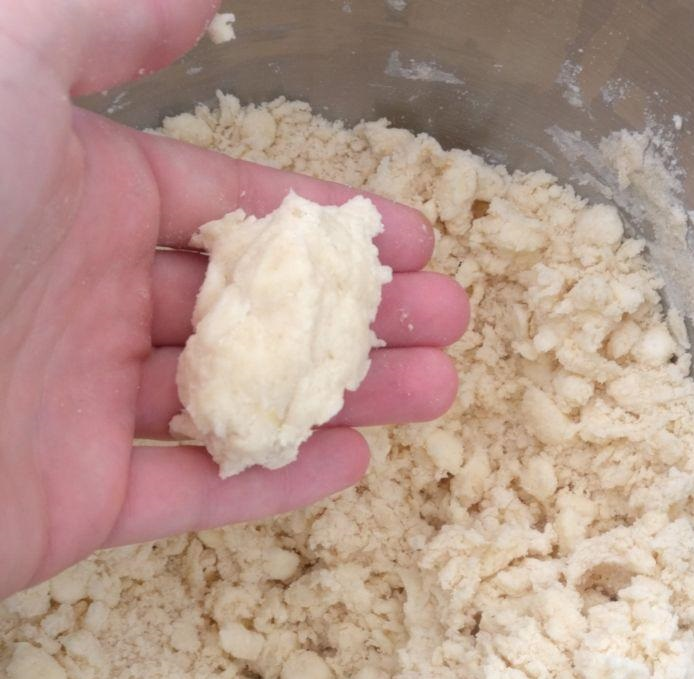
\includegraphics{images/pie-dough}}.

Gather all the crumbs together, just press them together, do not need the dough, into a square shape.
%
Cut it into four pieces, dust lightly with flour, and stack them together, to create some layers\sidenote{You can repeat this a couple or three times.}.
%
Wrap it\sidenote{Do you remember that reusable zip-lock bag?}, and put in the fridge for a at least a couple of hours.

\section{Baking}
Use some flour to open the dough with a rolling pin. 
%
Just put the dough in the tray and hit it with the filling, no need to bake before-hand. 
%
Egg-wash and sprinkle sugar on top.

Bake at $200^oC$ for about $30$ minutes, but keep and eye to not roast the top by putting it too close to the heat source. Ideally you have bottom heating as well.

\section{Experiments}
Instead of water, add something acidic, alcoholic, and possibly sweet to the dough. Great candidates are: Orange juice, White wine, and Cachaca.
%
The alcohol should evaporate during cooking, helping to keep the dough more crispy, while before cooking it helps to keep the dough "hydrated", making it easier to handle.
%
I guess the acid makes it harder to form gluten, resulting in a more flaky dough.

\section{Filling}

I personally like raw apples, with a bit of corn starch (by eye), and seasoning, in very low heat, without steering, to not brake the apples, but to remove some moist before putting in the dough to bake\sidenote{Avoid soggy-bottoms. Amen!}.
%
It a great use for the zast and rest of the juice used to hydrate the dough.

Great candidates are peaches, and berries in general, mind if they have too much water.

Now, you can also use this dough to savoury pies, by simply reducing the amount of sugar by half.

\pagelayout{wide} % No margins
\addpart{Technical}
\pagelayout{margin} % Restore margins

\setchapterstyle{kao}
\setchapterpreamble[u]{\margintoc}
\chapter{Pots, Compotes, and Long Lasting Stuff}\label{pots}


\section{Ingredients}

\begin{multicols}{2}
	\begin{description}
		\item[x] Glass pots with metal lid
		\item[Some] Stuff you want to preserve
	\end{description}
\end{multicols}	

\section{Preparation}
The stuff you want to preserve must be boiling hot, so it works only with cooked stuff.

Boil the pots and lids for $15$ minutes, add the stuff while super hot and boiling in the pots, and close them.

Return the pots to the boiling water for another $15$ minutes, for extra safety.

Leave the pots to cool down upside down. Store wherever, forever(-ish).

%----------------------------------------------------------------------------------------
%	BIBLIOGRAPHY
%----------------------------------------------------------------------------------------

% The bibliography needs to be compiled with biber using your LaTeX editor, or on the command line with 'biber main' from the template directory

\defbibnote{bibnote}{Here are the references in citation order.\par\bigskip} % Prepend this text to the bibliography
\printbibliography[heading=bibintoc, title=Bibliography, prenote=bibnote] % Add the bibliography heading to the ToC, set the title of the bibliography and output the bibliography note

%----------------------------------------------------------------------------------------
%	NOMENCLATURE
%----------------------------------------------------------------------------------------

% The nomenclature needs to be compiled on the command line with 'makeindex main.nlo -s nomencl.ist -o main.nls' from the template directory

\nomenclature{$c$}{Speed of light in a vacuum inertial frame}
\nomenclature{$h$}{Planck constant}

\renewcommand{\nomname}{Notation} % Rename the default 'Nomenclature'
\renewcommand{\nompreamble}{The next list describes several symbols that will be later used within the body of the document.} % Prepend this text to the nomenclature

\printnomenclature % Output the nomenclature


%----------------------------------------------------------------------------------------
%	GLOSSARY
%----------------------------------------------------------------------------------------

% The glossary needs to be compiled on the command line with 'makeglossaries main' from the template directory

\newglossaryentry{computer}{
	name=computer,
	description={is a programmable machine that receives input, stores and manipulates data, and provides output in a useful format}
}

% Glossary entries (used in text with e.g. \acrfull{fpsLabel} or \acrshort{fpsLabel})
\newacronym[longplural={Frames per Second}]{fpsLabel}{FPS}{Frame per Second}
\newacronym[longplural={Tables of Contents}]{tocLabel}{TOC}{Table of Contents}

\setglossarystyle{listgroup} % Set the style of the glossary (see https://en.wikibooks.org/wiki/LaTeX/Glossary for a reference)
\printglossary[title=Special Terms, toctitle=List of Terms] % Output the glossary, 'title' is the chapter heading for the glossary, toctitle is the table of contents heading

%----------------------------------------------------------------------------------------
%	INDEX
%----------------------------------------------------------------------------------------

% The index needs to be compiled on the command line with 'makeindex main' from the template directory

\printindex % Output the index

%----------------------------------------------------------------------------------------
%	BACK COVER
%----------------------------------------------------------------------------------------

% If you have a PDF/image file that you want to use as a back cover, uncomment the following lines

%\clearpage
%\thispagestyle{empty}
%\null%
%\clearpage
%\includepdf{cover-back.pdf}

%----------------------------------------------------------------------------------------

\end{document}
